% !Mode:: "TeX:UTF-8"
\definecolor{dkgreen}{rgb}{0,0.6,0}
\definecolor{gray}{rgb}{0.5,0.5,0.5}
\definecolor{mauve}{rgb}{0.58,0,0.82}

\lstset{frame=tb,
  language=Mathematica,
  aboveskip=3mm,
  belowskip=3mm,
  showstringspaces=false,
  columns=flexible,
  basicstyle={\small\ttfamily},
  numbers=left,
  numberstyle=\tiny\color{gray},
  keywordstyle=\color{blue},
  commentstyle=\color{dkgreen},
  stringstyle=\color{mauve},
  breaklines=true,
  breakatwhitespace=true
  tabsize=3
}
\chapter{ss方程守恒律程序包开发}
第二章第二节中介绍了偏微分方程的守恒律,守恒律作为非线性偏微分方程中一个很重要的性质,对于研究非线性偏微分来说具有很重要的作用。然而,求解偏微分方程守恒律的过程并不是一成不变的,一般来说不同类型方程的求解方式会具有很大的差异,在求解的过程中,往往只能凭借研究人员的个人的思考和过往研究经验对中间过程进行人工处理,才能得到最终的结果。幸运的是,在求解方程守恒律的过程中并不是所有的步骤都需要人工式的处理,仍然有一些步骤是机械式的流程,对于不同类型的方程,只要给出足够必要的条件,就能不断的迭代产生出从第一项到任意一项的守恒律。以 Sasa-Satsuma 方程为例,首先得到目标方程分别关于时间和空间多项式 $D_n$ 和 $F_n$ 的表达式,然后再得到表达式中依赖项的形式和起始项,就很容易的可以推导出任意一项的守恒律,最后进行验证是否正确。 因此可以将这一部分流程抽象出来,编写出用于求解守恒律的程序包。本章将主要介绍使用 Mathematica 内置的编程语言 Wolfram 来封装求解守恒律过程的程序包。

\section{Wolfram Mathematica 基本介绍}
Mathematica 是一款用于符号计算的软件,也被称为计算机代数系统,广泛用于科学研究、工程、数学计算等领域, 也是目前使用最为广泛的数学软件之一。而 Wolfram 语言是用于 Mathematica 的编程语言,它的用法和其它的高级编程语言有着很大的不同。Wolfram 集合了大量的编程模式,并使用独特的符号编程理念,是一种基于知识的语言,在编程上具有很大的灵活度。它使用各种语法规则去解释输入,使用标准输入框将字符串或框符转化为表达式。Wolfram 是一种交互式的编程语言,使用时只需敲入输入,然后按 SHIFT+ENTER 便可进行计算得到结果。下面将简要的介绍 Wolfram 语言中最基础的语法和概念。
\begin{itemize}
    \item 表达式
\end{itemize}

在 Wolfram 语言中,一切都是符号表达式。尽管 Wolfram 语言可以处理多种不同形式的对象,例如数学公式、列表、图形等,它们在形式上看起来有所不同,但是 Wolfram 语言以统一的方式来表达它们。符号表达式可以进一步的划分为两种类型:原子表达式和普通表达式。原子表达式是组成表达式中最小单元,主要包括数字、分数、实数、复数、符号、字符串等。普通表达式由原子表达式组成,所有的普通符号表达式都具有相同的基本结构:$head[arguments]$

${a, b, c} \cdots List[a, b, c]$

$2 + 2 \cdots Plus[2, 2]$

其中 $head$ 是表达式的头部, $arguments$ 表示表达式的参数,参数也可以是任何符号表达式,例如

$x^2 + 3y^3 \cdots Plus[Power[x, 2], Times[3, Power[y, 3]]]$

\begin{itemize}
   \item 列表
\end{itemize}

列表是 Wolfram 语言的一种重要的数据结构,用来表示各种类型的集合、数组以及序列。列表可以是任意的结构和大小,甚至包含数百万个元素。 Wolfram 语言可以直接在列表上操作的函数超过 1000 个,这使得列表成为 Mathematica 中一个协同工作的强大工具。在 Wolfram 语言中列表用 $\{\cdots\}$ 表示,其中的元素可以是任何类型的表达式。列表部分的索引从 1 开始,可以使用 $[[\cdots]]$ 进行提取,而负索引从列表的结尾向前开始计数,例如

$\{a, b, c\}[[3]]$ 的结果是 $c$,

$\{a, b, c, d, e, f\}[[-3]]$ 的结果是 $d$。
 
\begin{itemize}
    \item 函数
\end{itemize}

Wolfram 系统的符号语言模式,将变量和函数的定义提高到了一个新的层次。 在 Wolfram 系统中,变量不仅可以代表一个数值,而且可以作为一个纯粹的符号来使用。基于 Wolfram 系统强大的模式语言, “函数” 定义不仅仅是变量,而且可以转换为任意结构的模式。在 Wolfram 语言中,函数定义只是给出模式变换规则的复制,例如定义一个带有命名为 $x$ 和 $y$ 两个参数的函数

$f[x\_ , y\_ ]:= x + y$

使用上述定义

$f[4, a]$ 输出结果是 $4 + a$.

通常情况下,Wolfram 语言一般假设变量是全局变量. 即每次使用  $x$ 等名字时,Wolfram 语言总认为在调用同一对象。然而在编程时,不需要将所有变量都作为全局变量。例如,在两个不同的程序中,$x$ 可用来指代两个不同的变量. 此时,每个程序中的 $x$ 都必须作为局部变量。为了解决这个问题,在 Wolfram 语言中可以使用  Modules 定义局部变量,

$f[x\_ , y\_ ]:= (Module[\{x, y, \cdots\}, body])$

其中 $x, y$ 是局部变量,$body$ 处为具体的函数体

除了可以自定义函数外,Wolfram 语言还提供近 5000 个内置函数共用户使用,一般每个内置函数名称的首字母均为大写。这些内置函数会大大的简化程序编写的工作量,下面给出一些常用到的内置函数

$Simplify[expr]$  \quad   化简表达式 $expr$

$Expand[expr]$ \quad    展开表达式 $expr$ 的每一项

$Solve[expr, vars]$  \quad 求解以 $vars$ 为变量的方程组或不等式组 $expr$

$DSolve[eqn, u, x]$ \quad  为函数 $u$ 求解微分方程,$x$ 为独立变量

$DSolve[\{eqn_1, eqn_2, \cdots \}, \{u_1, u_2, \cdots \}, \cdots ]$ \quad  用来求解一系列微分方程

$D[f,x]$     \quad  关于函数 $f$ 对 $x$ 求微分

$D[f,{x,n}]$     \quad     关于函数 $f$ 求 $x$ 的 $n$ 阶微分

$Coefficient[expr, form]$   \quad  给出了多项式 $expr$ 中 $form$ 的系数

$CoefficientList[poly, var]$   \quad  给出在 $poly$ 中 $var$ 的幂系数的列表,从 0 次幂开始

\section{守恒律的求解实现}
如果知道一个微分方程的守恒律的表达式以及表达式依赖项的形式和起始项,那么我们就可以求出该方程任意一组的守恒律,当然首先是需要得到守恒律的通项公式。

以下是代码的简单实现
\begin{lstlisting}[language=Mathematica,caption=变量变换方法的实现]

\end{lstlisting}


\section{验证怪波解}
上一节实现了两个方程的变量变换,接下来将变量变换关系应用于方程的已知怪波解,就能得到另一个方程的怪波解,并且进行验证。具体实现代码如下:

\begin{lstlisting}[language=Mathematica,caption=验证怪波解]
(*将第一个方程到第二个方程的变量变换的结果应用到第二个方程的怪波解上可以得到第一个方程的怪波解*)
(*X T A 分别是前一步变量变换求得的结果*)
(*equ第一个方程,即最后我们要验证怪波解的方程*)
DeRogue[X_,T_,A_,equ_]:=(Module[{d,c,k},
d=1;
c=1;
k=1;
a2[t]=m a5[t];
K=1+3k;
u0[x,t]=-A c/(2d) Exp[-I/(2d) (k X-w/(4d) T)];
v0[x,t]=-A c/(2d) Exp[I/(2d) (k X-w/(4d) T)];
w=2c^2 (1+3k)-k^2-k^3;
G=(d^2 (9c^2+2K^2))/(2c^2 K^2) (a+(4k1^2 k2^2)/(9c^2+2K^2) T)^2+(8d^2 k1^2 k2^2 (k1^2-k2^2))/(c^2 (9c^2+2K^2)) T^2+(162d^6 (9c^2+2K^2)^3)/(c^2 k1^2 k2^2 (k1^2+k2^2)^2);
H=1/(2K) (a^2/4+k1^2 k2^2 T^2-(243d^4 (9c^2+2K^2)^2)/(k1^2 k2^2 (18c^2+K^2)))(a+(4k1^2 k2^2)/(9c^2) T)+(16d^4 k1^2 k2^2 (27c^2+2K^2))/(c^4 K(18c^2+K^2)) T;
B=1/(36d^2) (a^2/4+k1^2 k2^2 T^2+(18^2 d^4 (k1^4-k1^2 k2^2-k2^4))/(k1^2 k2^2 (k1^2+k2^2)))^2+(9d^2 k2^2)/(k1^2+k2^2)^2 (a+2k1^2 T)^2+(108^2 d^6)/(k2^2 (k1^2+k2^2));
a=(K^2-1-27c^2)T+12d X;
k1=Sqrt[2]/2 (Sqrt[K^2 (18c^2+K^2)]-9c^2+K^2)^(1/2);
k2=Sqrt[2]/2 (Sqrt[K^2 (18c^2+K^2)]+9c^2-K^2)^(1/2);
u[x,t]=u0[x,t](1-(G+I H)/B);
v[x,t]=v0[x,t](1-(G-I H)/B);
Simplify[equ]
])
\end{lstlisting}
$DeRogue$ 函数接收四个变量,$X, T, A$ 是前一步求出的变量变换中假设变量的值,$equ$ 是要求解怪波解的方程。$u0[x,t]$ 和 $v0[x,t]$ 是简单方程的平波解,$u[x,t]$ 和 $v[x,t]$ 是简单方程的怪波解,将变量变换的关系式代入就能得到复杂方程的怪波解,最后对复杂方程的怪波解进行验证,如果最后输出的结果为零,则怪波解求解成功。上面已经求到了方程 (\ref{ss-9}) 到方程 (\ref{ss-1}) 变量变换的关系表达式,接下来继续代入求怪波解并进行验证。
\begin{figure}[!htp]
	\centering
	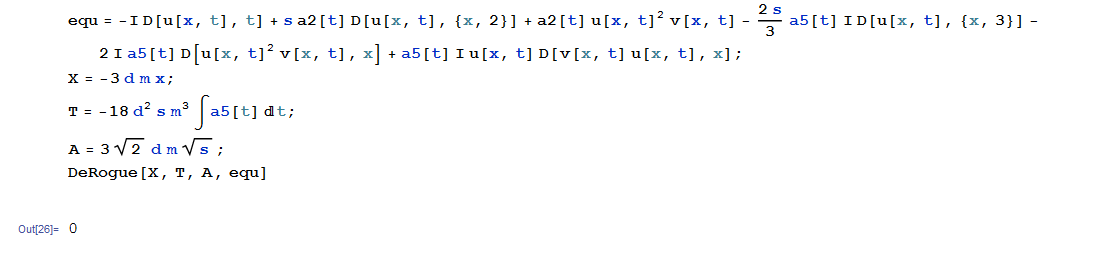
\includegraphics[width=\linewidth]{rogueResult.jpg}
	\caption{验证怪波运行结果}
	%with same parameters~$k=1 , \alpha_2(t)=1, \alpha_0(t)=0$.
	\label{}
\end{figure}
$X, T, A$ 是上一步变量变换得到的结果,$equ$ 是方程 (\ref{ss-1}) 的表达式,将变量变换后的怪波解代入 $equ$ 输出结果为零,完成验证。
\section{本章小结}
本章首先介绍了 Mathematica 内置 Wolfram 语言的基本语法、常用函数的用法与含义,然后用 Wolfram 封装了根据已知方程的怪波解得到另一方程的怪波解的过程。这个过程主要分为两个部分,第一,找到两个方程的变量变换的关系表达式,即 $DeReplace$ 函数的实现;第二,将变量变换的关系表达式代入已知的怪波解就可以得到另一方程的怪波解,并进行了验证,即 $DeRogue$ 函数的实现。最后,可以看到本章通过间接法得到的怪波解与第三章用 Darboux 变换法直接法求得的怪波解一致,变量变换为同一类型的方程的研究提供了捷径,也为求解怪波解提供了一个新思路。


